\begin{problem}[IMO 2019 SL - Problem C4]
On a flat plane in Camelot, King Arthur builds a labyrinth \( L \) consisting of \( n \) walls, each of which is an infinite straight line. No two walls are parallel, and no three walls have a common point. Merlin then paints one side of each wall entirely red and the other side entirely blue.

At the intersection of two walls there are four corners: two diagonally opposite corners where a red side and a blue side meet, one corner where two red sides meet, and one corner where two blue sides meet. At each such intersection, there is a two-way door connecting the two diagonally opposite corners at which sides of different colours meet.

After Merlin paints the walls, Morgana then places some knights in the labyrinth. The knights can walk through doors, but cannot walk through walls.

Let \( k_p(L) \) be the largest number \( k \) such that, no matter how Merlin paints the labyrinth \( L \), Morgana can always place at least \( k \) knights such that no two of them can ever meet. For each \( n \), what are all possible values for \( k_p(L) \), where \( L \) is a labyrinth with \( n \) walls?
\end{problem}

\textbf{Answer:} The only possible value of \( k \) is \( n + 1 \), no matter what shape the labyrinth is.

\section*{Solution 1.}

First we show by induction that the \( n \) walls divide the plane into \( \frac{n(n+1)}{2} \) regions.

The claim is true for \( n = 0 \) as, when there are no walls, the plane forms a single region. When placing the \( n \)th wall, it intersects each of the \( n - 1 \) other walls exactly once and hence splits each of \( n \) of the regions formed by those other walls into two regions. By the induction hypothesis, this yields 
\[
\frac{n(n-1)}{2} + 1 + n = \frac{n(n+1)}{2} + 1
\]
regions, proving the claim.

Now let \( G \) be the graph with vertices given by the \( \frac{n(n+1)}{2} + 1 \) regions, and with two regions connected by an edge if there is a door between them.

We now show that no matter how Merlin paints the \( n \) walls, Morgana can place at least \( n + 1 \) knights. No matter how the walls are painted, there are exactly 
\[
\frac{n(n-1)}{2} = \binom{n}{2}
\]
intersection points, each of which corresponds to a single edge in \( G \). Consider adding the edges of \( G \) sequentially and note that each edge reduces the number of connected components by at most one. Therefore the number of connected components of \( G \) is at least
\[
\left( \binom{n+1}{2} + 1 \right) - \binom{n}{2} = n + 1.
\]
If Morgana places a knight in regions corresponding to different connected components of \( G \), then no two knights can ever meet. 

Now we give a construction showing that, no matter what shape the labyrinth is, Merlin can colour it such that there are exactly \( n + 1 \) connected components, allowing Morgana to place at most \( n + 1 \) knights. 

First, we choose a coordinate system on the labyrinth so that none of the walls run due north-south, or due east-west. We then have Merlin paint the west face of each wall red, and the east face of each wall blue. We label the regions according to how many walls the region is on the east side of: the labels are integers between \( 0 \) and \( n \).

We claim that, for each \( i \), the regions labelled \( i \) are connected by doors. First, we note that for each \( i \) with \( 0 \leq i \leq n \), there is a unique region labelled \( i \) which is unbounded to the north.

Now, consider a knight placed in some region with label \( i \), and ask them to walk north (moving east or west by following the walls on the northern sides of regions, as needed). This knight will never get stuck: each region is convex, and so, if it is bounded to the north, it has a single northernmost vertex with a door northwards to another region with label \( i \).

Eventually it will reach a region which is unbounded to the north, which will be the unique such region with label \( i \). Hence every region with label \( i \) is connected to this particular region, and so all regions with label \( i \) are connected to each other.

As a result, there are exactly \( n + 1 \) connected components, and Morgana can place at most  \( n + 1 \) knights. 

\section*{Solution 2.}

We give another description of a strategy for Merlin to paint the walls so that Morgana can place no more than \( n + 1 \) knights. 

Merlin starts by building a labyrinth of \( n \) walls of his own design. He places walls in turn with increasing positive gradients, placing each so far to the right that all intersection points of previously-placed lines lie to the left of it. He paints each in such a way that blue is on the
left and red is on the right. 

For example, here is a possible sequence of four such lines \( \ell_1, \ell_2, \ell_3, \ell_4 \):

\begin{center}
    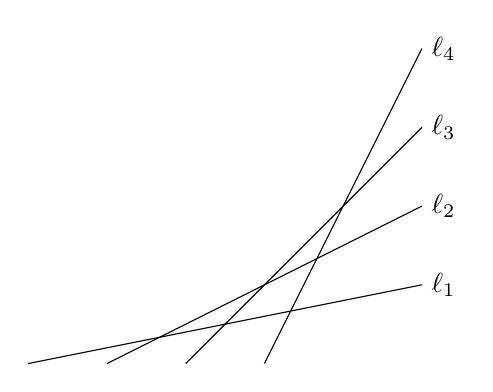
\begin{tikzpicture}[x=1cm,y=1cm]
    
    % \draw[->] (-1,0) -- (4,0)   node[right] {$x$};
    % \draw[->] (0,-1) -- (0,4)   node[above] {$y$};

    \draw (-1,0) -- (4,1) node[anchor=west]{$\ell_1$};
    \draw (0,0) -- (4,2) node[anchor=west]{$\ell_2$};
    \draw (1,0) -- (4,3) node[anchor=west]{$\ell_3$};
    \draw (2,0) -- (4,4) node[anchor=west]{$\ell_4$};
    \end{tikzpicture}
\end{center}

We say that a region is ``on the right'' if it has \( x \)-coordinate unbounded above (note that if we only have one wall, then both regions are on the right). We claim inductively that, after placing \( n \) lines, there are \( n + 1 \) connected components in the resulting labyrinth, each of which contains exactly one region on the right. This is certainly true after placing \( 0 \) lines, as then there is only one region (and hence one connected component) and it is on the right. When placing the \( n \)th line, it then cuts every one of the \( n - 1 \) previously placed lines, and since it is to the right of all intersection points, the regions it cuts are exactly the \( n \) regions on the right.

\begin{center}
    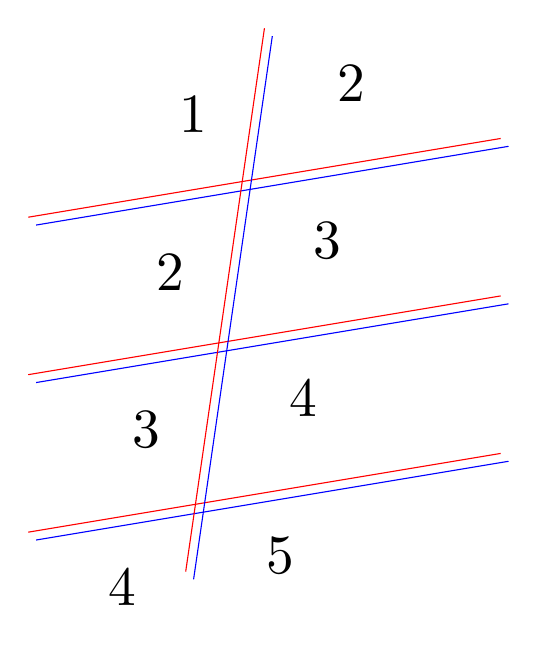
\begin{tikzpicture}[scale=2, every node/.style={transform shape}]
        \foreach \i in {1,2,3} {
            \draw[blue] (-1,\i) -- (2,\i+0.5);
            \draw[red,shift={(-0.05,0.05)}] (-1,\i) -- (2,\i+0.5);
        }

        \draw[blue] (0.5,4.2) -- (0, 0.75);
        \draw[red,shift={(-0.05,0.05)}] (0.5,4.2) -- (0, 0.75);

        \node at (0,3.7) {1};
        \node at (1,3.9) {2};

        \node[shift={(-0.15,-1)}] at (0,3.7) {2};
        \node[shift={(-0.15,-1)}] at (1,3.9) {3};

        \node[shift={(-0.3,-2)}] at (0,3.7) {3};
        \node[shift={(-0.3,-2)}] at (1,3.9) {4};

        \node[shift={(-0.45,-3)}] at (0,3.7){4};
        \node[shift={(-0.45,-3)}] at (1,3.9){5};
        
    \end{tikzpicture}
\end{center}

The addition of this line leaves all previous connected components with exactly one region on the right, and creates a new connected component containing exactly one region, and that region is also on the right. As a result, by induction, this particular labyrinth will have \( n + 1 \) connected components. Having built this labyrinth, Merlin then moves the walls one-by-one (by a sequence of continuous translations and rotations of lines) into the proper position of the given labyrinth, in such a way that no two lines ever become parallel.

The only time the configuration is changed is when one wall is moved through an intersection point of two others:

\begin{figure}[h]
    \centering
    \captionsetup{labelformat=empty}
    \begin{subfigure}[b]{0.45\textwidth}
        \centering
        \captionsetup{labelformat=empty}
        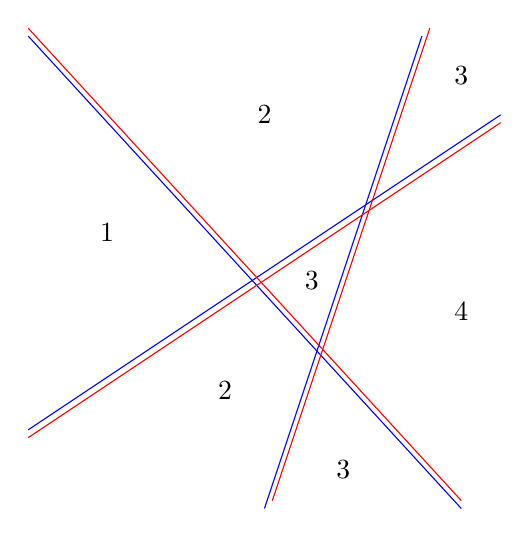
\begin{tikzpicture}
            \draw[blue] (2, 8) -- (7.5, 2);
            \draw[blue] (2, 3) -- (8, 7);
            \draw[blue] (7, 8) -- (5, 2);

            \draw[red, shift={(0,0.1)}] (2, 8) -- (7.5, 2);
            \draw[red, shift={(0,-0.1)}] (2, 3) -- (8, 7);
            \draw[red, shift={(0.1,0.1)}] (7, 8) -- (5, 2);

            \node at (3, 5.5){1} ;
            \node at (5, 7){2};
            \node at (4.5, 3.5){2} ;
            \node at (5.6, 4.9){3} ;
            \node at (7.5, 7.5){3} ;
            \node at (6, 2.5){3} ;
            \node at (7.5, 4.5){4} ;
    \end{tikzpicture}
    \end{subfigure}
    \hfill
    \begin{subfigure}[b]{0.45\textwidth}
        \centering
        \captionsetup{labelformat=empty}
        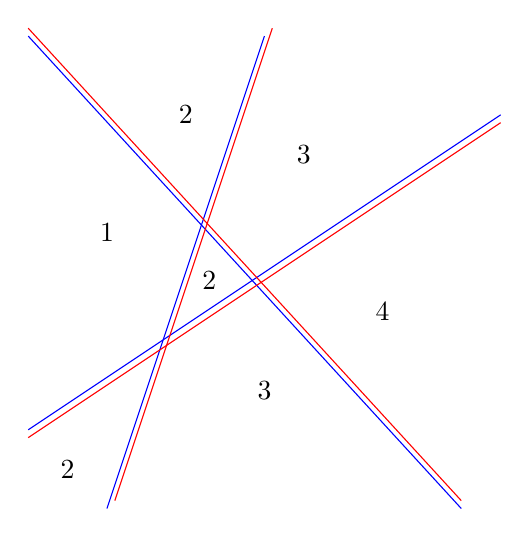
\begin{tikzpicture}
            \draw[blue] (2, 8) -- (7.5, 2);
            \draw[blue] (2, 3) -- (8, 7);
            \draw[blue,shift={(-2,0)}] (7, 8) -- (5, 2);

            \draw[red, shift={(0,0.1)}] (2, 8) -- (7.5, 2);
            \draw[red, shift={(0,-0.1)}] (2, 3) -- (8, 7);
            \draw[red, shift={(-1.9,0.1)}] (7, 8) -- (5, 2);

            \node at (3, 5.5){1} ;
            \node[shift={(-1,0)}] at (5, 7){2};
            \node[shift={(-2,-1)}] at (4.5, 3.5){2} ;
            \node[shift={(-1.3,0)}] at (5.6, 4.9){2} ;
            \node[shift={(-2,-1)}] at (7.5, 7.5){3} ;
            \node at (5, 3.5){3} ;
            \node at (6.5, 4.5){4} ;
        \end{tikzpicture}
    \end{subfigure}
\end{figure}

Note that all moves really do switch between two configurations like this: all sets of three lines have this colour configuration initially, and the rules on rotations mean they are preserved (in particular, we cannot create three lines creating a triangle with three red edges inwards, or three blue edges inwards). However, as can be seen, such a move preserves the number of connected components, so in the painting this provides for Arthur’s actual labyrinth, Morgana can still only place at most \( n + 1 \) knights.